% Options for packages loaded elsewhere
\PassOptionsToPackage{unicode}{hyperref}
\PassOptionsToPackage{hyphens}{url}
%
\documentclass[
  12pt,
]{article}
\usepackage{amsmath,amssymb}
\usepackage{iftex}
\ifPDFTeX
  \usepackage[T1]{fontenc}
  \usepackage[utf8]{inputenc}
  \usepackage{textcomp} % provide euro and other symbols
\else % if luatex or xetex
  \usepackage{unicode-math} % this also loads fontspec
  \defaultfontfeatures{Scale=MatchLowercase}
  \defaultfontfeatures[\rmfamily]{Ligatures=TeX,Scale=1}
\fi
\usepackage{lmodern}
\ifPDFTeX\else
  % xetex/luatex font selection
  \setmainfont[]{Arial}
\fi
% Use upquote if available, for straight quotes in verbatim environments
\IfFileExists{upquote.sty}{\usepackage{upquote}}{}
\IfFileExists{microtype.sty}{% use microtype if available
  \usepackage[]{microtype}
  \UseMicrotypeSet[protrusion]{basicmath} % disable protrusion for tt fonts
}{}
\makeatletter
\@ifundefined{KOMAClassName}{% if non-KOMA class
  \IfFileExists{parskip.sty}{%
    \usepackage{parskip}
  }{% else
    \setlength{\parindent}{0pt}
    \setlength{\parskip}{6pt plus 2pt minus 1pt}}
}{% if KOMA class
  \KOMAoptions{parskip=half}}
\makeatother
\usepackage{xcolor}
\usepackage[margin=1in]{geometry}
\usepackage{longtable,booktabs,array}
\usepackage{calc} % for calculating minipage widths
% Correct order of tables after \paragraph or \subparagraph
\usepackage{etoolbox}
\makeatletter
\patchcmd\longtable{\par}{\if@noskipsec\mbox{}\fi\par}{}{}
\makeatother
% Allow footnotes in longtable head/foot
\IfFileExists{footnotehyper.sty}{\usepackage{footnotehyper}}{\usepackage{footnote}}
\makesavenoteenv{longtable}
\usepackage{graphicx}
\makeatletter
\def\maxwidth{\ifdim\Gin@nat@width>\linewidth\linewidth\else\Gin@nat@width\fi}
\def\maxheight{\ifdim\Gin@nat@height>\textheight\textheight\else\Gin@nat@height\fi}
\makeatother
% Scale images if necessary, so that they will not overflow the page
% margins by default, and it is still possible to overwrite the defaults
% using explicit options in \includegraphics[width, height, ...]{}
\setkeys{Gin}{width=\maxwidth,height=\maxheight,keepaspectratio}
% Set default figure placement to htbp
\makeatletter
\def\fps@figure{htbp}
\makeatother
\setlength{\emergencystretch}{3em} % prevent overfull lines
\providecommand{\tightlist}{%
  \setlength{\itemsep}{0pt}\setlength{\parskip}{0pt}}
\setcounter{secnumdepth}{-\maxdimen} % remove section numbering
\ifLuaTeX
  \usepackage{selnolig}  % disable illegal ligatures
\fi
\usepackage{bookmark}
\IfFileExists{xurl.sty}{\usepackage{xurl}}{} % add URL line breaks if available
\urlstyle{same}
\hypersetup{
  pdfauthor={Nick Xing: Section 2, combining files; Zihan Zhu: Sections 3 \& 4; Noah Clark: Cover Page \& Section 1},
  hidelinks,
  pdfcreator={LaTeX via pandoc}}

\title{Hospital Insurance Charges Model \vspace{0.5cm}\\
Final for STAT 425}
\author{Nick Xing: Section 2, combining files \and Zihan Zhu: Sections 3
\& 4 \and Noah Clark: Cover Page \& Section 1}
\date{May 6, 2024}

\begin{document}
\maketitle

{
\setcounter{tocdepth}{3}
\tableofcontents
}
\newpage

\subsection{Section 1: Introduction}\label{section-1-introduction}

This project focuses on the analysis of medical insurance data,
particularly focusing on the medical charges acquired from hospital
visits. The response variable is the variable charges from the insurance
data. This data is found on Kaggle, as was last updated 6 years ago, in
2018. In this data set, there 6 variables excluding the response
variable, charges, which shows the exact charges the patient acquired
from their hospital visit. Each variable is defined within the Kaggle
(2018) website and explained in this order:

\begin{itemize}
\item
  age: Age of primary beneficiary
\item
  sex: Insurance contractor gender (female or male)
\item
  bmi: Body mass index, providing an understanding of body, weights that
  are relatively high or low relative to height, objective index of body
  weight (kg / m \^{} 2) using the ratio of height to weight, ideally
  18.5 to 24.9
\item
  children: Number of children covered by health insurance / Number of
  dependents
\item
  smoker: Smoking (yes or no)
\item
  region: Beneficiary's residential area in the US (northeast,
  southeast, southwest, northwest)
\item
  charges: Individual medical costs billed by health insurance
\end{itemize}

This report compares multiple models derived from analysis of the data
set including a Regression Model, an a Ridge Model, and a Lasso Model.
All analyses are performed in the R environment. This is possible to
recreate with the code provided in this file. Setting seeds might yield
slightly different results; however, we did not use a seed to analyze
this data. No function (i.e.~\emph{set.seed}) should change the results
concluded from this data, although it is possible to slightly alter the
data using said functions. Again, the results would be concluded the
same way. This report has 4 sections. Section 1 is this introduction.
Section 2 uses modelling assumptions and models to analyze the data and
provide insights on the data. Section 3 presents predictive models and
shows training from said models. Section 4 compares models and provides
a discussion of these results.

\newpage

\subsection{Section 2: Exploratory Data
Analysis}\label{section-2-exploratory-data-analysis}

Here is a brief overview of all of the variables of this dataset:

Numerical Variables:

\begin{itemize}
\tightlist
\item
  age: age of primary beneficiary
\item
  bmi: body mass index
\item
  children: number of children/dependents covered by health insurance
\item
  charges (response variable): medical costs billed by health insurance
\end{itemize}

Categorical Variables:

\begin{itemize}
\tightlist
\item
  sex: male or female
\item
  smoker: yes or no
\item
  region: residential area in the US, can be northeast, southeast,
  southwest, or northwest
\end{itemize}

The first step is to check for unusual observations by performing an
outlier test. To do so, we obtained the studentized residuals for our
data, and compared the largest values with the Bonferroni critical
value.

The Bonferroni critical value we calculated is -4.137174. Any
observation with studentized residual higher than the absolute value of
it will be considered an outlier.

Next, here are the five largest studentized residuals, which we will be
comparing to the Bonferroni critical value:

\begin{longtable}[]{@{}lr@{}}
\toprule\noalign{}
& x \\
\midrule\noalign{}
\endhead
\bottomrule\noalign{}
\endlastfoot
1301 & 5.009599 \\
578 & 4.219800 \\
243 & 4.053228 \\
220 & 3.998326 \\
517 & 3.863878 \\
\end{longtable}

Since the absolute value of their respective studentized residual is
greater than the Bonferroni critical value, we can conclude that
Observation \#1301 and Observation \#578 are outliers.

We also checked Cook's distance, however we found that there is no point
with Cook's distance greater than 1. We will simply remove the two
outliers we found earlier.

\newpage

After removing these two points, we will be analyzing the predictors to
see if there are any variables we should add or remove.

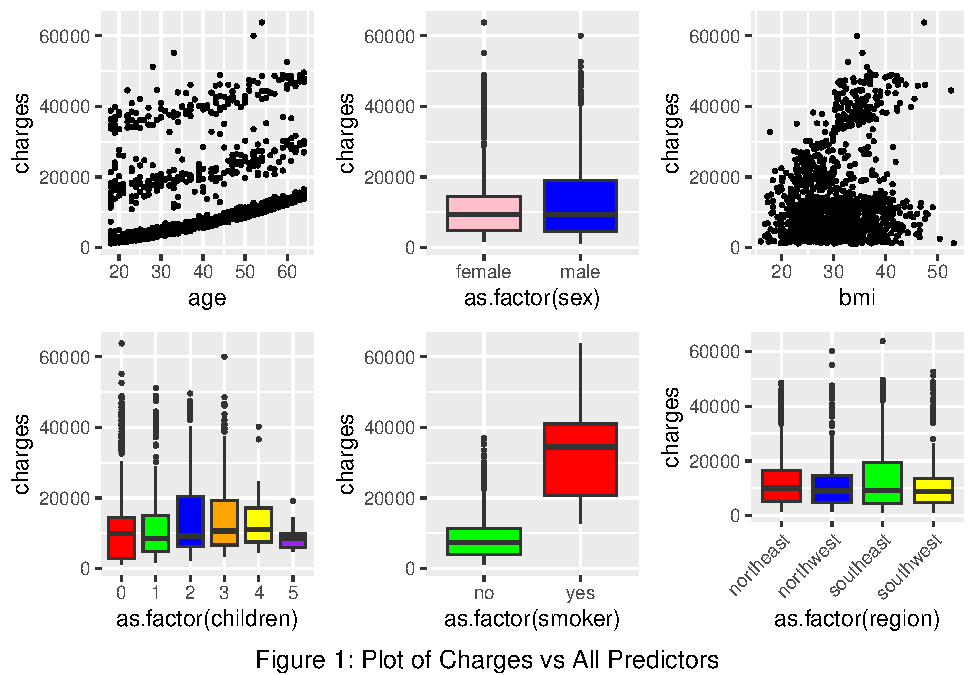
\includegraphics{finalproject_files/figure-latex/unnamed-chunk-7-1.pdf}

From the plot of charges vs age, we notice a trend that the charges
increase as age increases. We will not be removing `age' as a predictor
since it is clear that it has a significant impact on the response
variable `charges'. This makes sense because as people grow older, their
health declines, and the insurance costs increase.

The charges vs sex boxplot tells us that males tend to have higher
charges than females. We will conduct a t-test to test this difference.

From the t-test, we obtained a p-value of about 0.0346.

Given that the p-value is less than 0.05, we conclude that `sex' is a
significant predictor, with males incurring higher insurance costs than
females. A possible explanation for this is that males are usually more
at risk of health conditions that result in increased charges compared
to females.

From the plot of charges vs bmi, we can see a general trend that as bmi
increases, the charges also increase. As a result, we will not be
removing `bmi' as a predictor since it appears to have an impact on the
response variable. The graph also makes sense logically since people
with a higher bmi tend to be overweight and subsequently, have worse
health than people with a lower bmi, causing their insurance charges to
be greater as well.

The boxplot of charges vs children conveys to us that charges tend to
increase as the number of children grows from 0 or 1 to 2 or 3. While
there are some data points for people with 4 or 5 children, it appears
that these groups have a very low amount of people, and it may be
challenging to draw meaningful conclusions from it. We perform an ANOVA
test to test the significance of `children' as a predictor.

We obtained a p-value of approximately 0.00862.

This p-value is less than 0.05, thus signifying that the predictor
`children' is significant. We will be keeping as a predictor in our
model. A larger number of children/dependents covered leads to higher
charges, as there are more individuals who need to be covered.

From the boxplot of charges vs smoker, it is evident that smokers
generally face significantly higher charges than non-smokers.
Consequently, we will not be removing `smoker' as a predictor. People
who smoke typically incur higher insurance costs due to the health risks
posed by smoking.

The boxplot of charges vs region shows us that the southeast region
seemingly has higher charges than the other three regions. We will
conduct an ANOVA test to make sure that the predictor `region' is
significant.

From the ANOVA test, we obtained a p-value of about 0.0453.

The p-value is less than 0.05, indicating that the predictor `region' is
significant, and thus we will retain it as a predictor. This confirms
that there are regional differences in the insurance costs.

\newpage

Now, we will explore whether or not we should include any interactions
between categorical variables. We will be analyzing all possible
first-order and second-order interactions between our categorical
predictors, including:

\begin{itemize}
\tightlist
\item
  `sex' and `smoker'
\item
  `sex' and `region'
\item
  `region' and `smoker'
\item
  `sex', `smoker', and `region'
\end{itemize}

Here are some plots that show the interactions between these predictors.

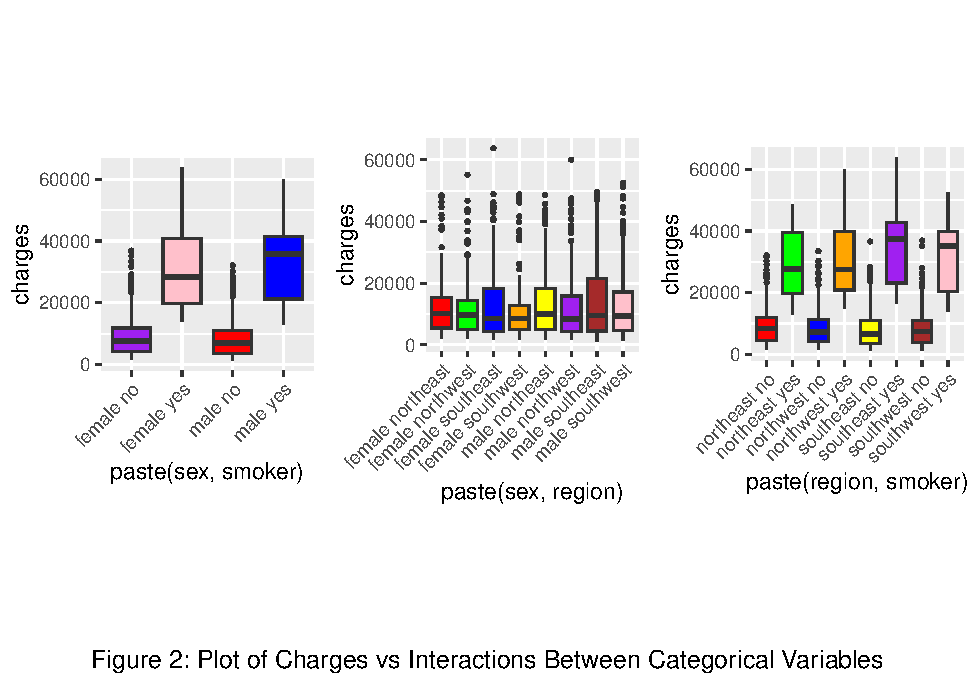
\includegraphics{finalproject_files/figure-latex/unnamed-chunk-11-1.pdf}

From the plots, it appears as though smoking increases the charges more
for males than females. Additionally, it seems like smoking has a
greater impact on charges in the southeast and southwest, when compared
to northeast and northwest. However, it does not appear that sex and
region is a significant interaction.

We applied sequential F-tests with the anova function to assess the
significance of the interaction terms in our model. Initially, we
included all potential interactions among the three variables `sex',
`smoker', and `region'. We first found that the second-order interaction
sex:smoker:region was not significant, and removed it from the model.
Subsequently, we tested the first-order interactions and found that the
interaction sex:region was not significant. Finally, after removing
sex:region as a predictor, we concluded that only the interactions
sex:smoker and smoker:region are statistically significant, and we will
retain them in the final model.

Now, we will examine the numerical variables and see if there is
evidence of any nonlinear trends.

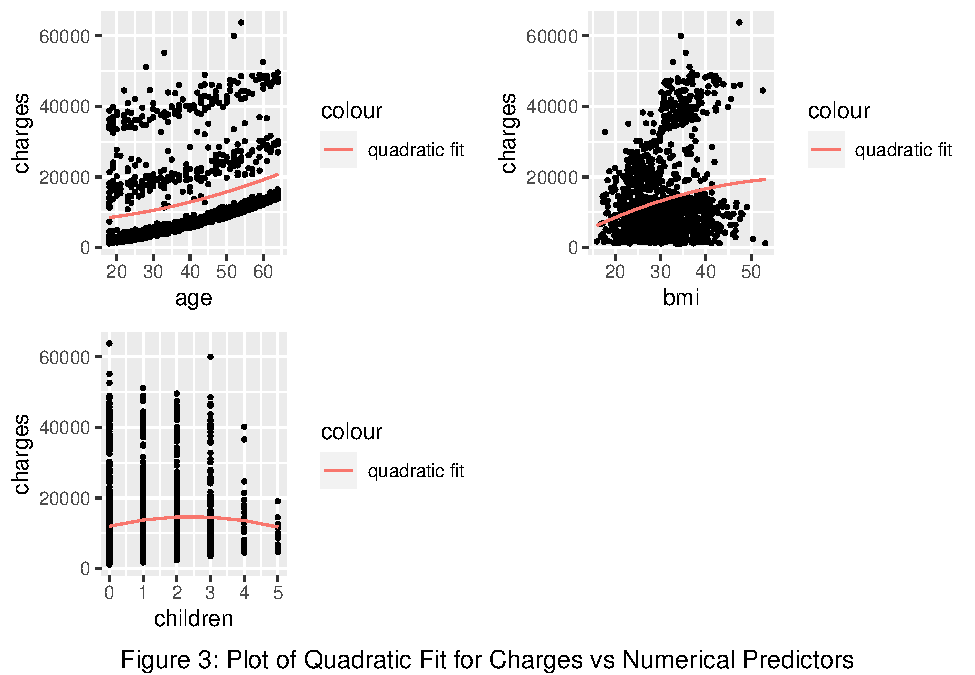
\includegraphics{finalproject_files/figure-latex/unnamed-chunk-16-1.pdf}

Based on the plot of the quadratic fit for charges vs age, we see there
is evidence of non-linearity for the predictor `age' since the quadratic
fit has some upward curvature.

Similarly, based on the plot of the quadratic fit for charges vs bmi, we
see there is some evidence of non-linearity for the predictor `bmi',
although maybe not as clear as for `age'. This time, the quadratic fit
curves downwards.

Finally, the plot of charges vs children also suggests some
non-linearity. However, the non-linearity is not as evident as for `age
and 'bmi' since although the quadratic fit does appear to curve
downwards as the number of children increases, there is not many data
points for 4 and 5 children, so we may not be able to draw a strong
conclusion.

\newpage

\subsection{Section 3: Methodology}\label{section-3-methodology}

\subsubsection{Section 3.1: Simple
Model}\label{section-3.1-simple-model}

Model Selection The choice of linear regression for this analysis is
based on its efficacy in providing a clear and straightforward
interpretation of how various predictors affect insurance charges.
Linear regression is particularly valued for its ability to establish a
baseline understanding of the relationships between variables, offering
insights into the direct impacts of age, BMI, children count, smoking
status,sex and regional differences on insurance costs. Variable
Selection and Diagnostics Age: A continuous variable expected to
positively correlate with insurance charges. BMI: Another continuous
variable, which is hypothesized to influence insurance costs due to its
association with health risks. Children: A discrete variable that
represents the number of dependents,potentially affecting insurance
premiums. Smoker Status: A categorical variable that significantly
impacts insurance costs, as identified in the exploratory analysis.
Sex:A categorical variable, often considered in insurance cost analysis
because gender may influence health risks and insurance premiums.
Region: As a categorical variable, the region captures variations in
insurance costs across different geographical locations. Sex and Smoker
Interaction: This interaction term examines how gender and smoking
status jointly influence insurance costs. Smokers of different genders
may face different health risks, which can be reflected in their
insurance premiums. Region and Smoker Interaction: This interaction term
was included to examine if the impact of smoking on insurance charges
varies by region, which could suggest regional variations in healthcare
costs or lifestyle patterns.

\begin{longtable}[]{@{}lrrr@{}}
\toprule\noalign{}
& GVIF & Df & GVIF\^{}(1/(2*Df)) \\
\midrule\noalign{}
\endhead
\bottomrule\noalign{}
\endlastfoot
age & 1.017141 & 1 & 1.008534 \\
bmi & 1.108041 & 1 & 1.052635 \\
children & 1.004025 & 1 & 1.002011 \\
smoker & 1.011905 & 1 & 1.005935 \\
sex & 1.009150 & 1 & 1.004565 \\
region & 1.099632 & 3 & 1.015955 \\
\end{longtable}

\begin{verbatim}
## 
## Call:
## lm(formula = charges ~ age + bmi + children + smoker + sex + 
##     region + sex:smoker + smoker:region, data = insurance2)
## 
## Residuals:
##    Min     1Q Median     3Q    Max 
## -13669  -2817  -1035   1269  25874 
## 
## Coefficients:
##                            Estimate Std. Error t value Pr(>|t|)    
## (Intercept)               -10872.78     980.81 -11.085  < 2e-16 ***
## age                          256.73      11.57  22.197  < 2e-16 ***
## bmi                          329.46      27.84  11.836  < 2e-16 ***
## children                     493.41     133.85   3.686 0.000237 ***
## smokeryes                  19484.22     931.12  20.926  < 2e-16 ***
## sexmale                     -600.93     360.92  -1.665 0.096153 .  
## regionnorthwest             -506.43     514.05  -0.985 0.324713    
## regionsoutheast            -2272.77     524.14  -4.336 1.56e-05 ***
## regionsouthwest            -1748.10     515.09  -3.394 0.000710 ***
## smokeryes:sexmale           2163.42     812.25   2.663 0.007827 ** 
## smokeryes:regionnorthwest    978.98    1178.49   0.831 0.406291    
## smokeryes:regionsoutheast   5661.02    1082.02   5.232 1.95e-07 ***
## smokeryes:regionsouthwest   4329.60    1178.69   3.673 0.000249 ***
## ---
## Signif. codes:  0 '***' 0.001 '**' 0.01 '*' 0.05 '.' 0.1 ' ' 1
## 
## Residual standard error: 5881 on 1323 degrees of freedom
## Multiple R-squared:  0.7612, Adjusted R-squared:  0.759 
## F-statistic: 351.4 on 12 and 1323 DF,  p-value: < 2.2e-16
\end{verbatim}

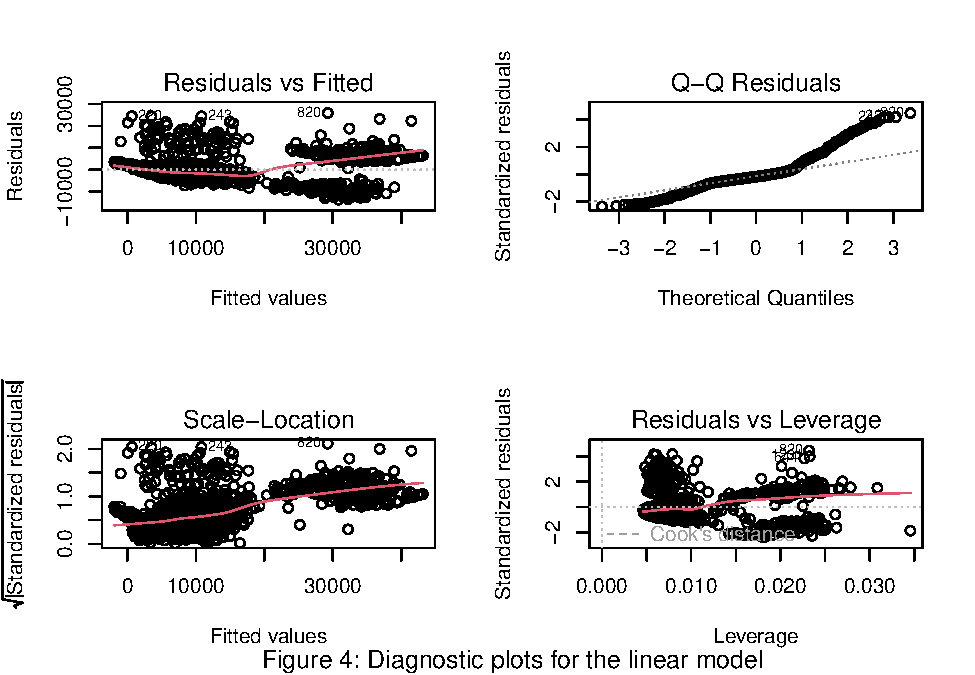
\includegraphics{finalproject_files/figure-latex/unnamed-chunk-19-1.pdf}
Model Diagnostics: The diagnostics conducted include: Multicollinearity
Check: The Variance Inflation Factor (VIF) was calculated for all
predictors, with results indicating minimal multicollinearity among the
variables used. VIF values were as follows: age (1.00), BMI(1.05),
children (1.00), smoker status (1.01), sex (1.00) and region(1.02).
Model Fit: The linear model was fitted with charges as the dependent
variable. The R-squared value of 0.7612 suggests that about 76.12\% of
the variability in insurance charges is explained by the model, which is
quite substantial for a simple linear model.

Residual Analysis: Residuals: The residuals' plot indicated that while
there is some spread, major deviations from normality or constant
variance (homoscedasticity) were not apparent, suggesting that the model
assumptions are reasonably met.

Coefficients: Intercept: The model's intercept is significantly
negative, which might indicate that the baseline insurance charges are
negative when all other variables are zero. This could suggest that
further adjustments to the model might be necessary.

Age: The coefficient for age is significant and positive, indicating
that insurance charges increase with age. This aligns with the general
logic of insurance pricing, where increased age is associated with
higher health risks.

BMI: The coefficient for BMI is also significantly positive, suggesting
that higher BMI is associated with higher insurance charges, likely due
to increased health risks associated with higher BMI.

Children: The coefficient for the number of children is significant and
positive, indicating that having more children leads to higher insurance
charges, possibly reflecting the greater healthcare needs of larger
families.

Significant Impact of Smoking Status: The coefficient for smokers is
significantly higher than for non-smokers, consistent with previous
studies indicating that smoking is a significant factor affecting
insurance costs.

Interactions of Region and Gender: Region Coefficients: Some regional
categories, such as southeast and southwest, are significant, suggesting
that insurance costs in these regions are higher compared to the
baseline region.

Interaction of Smoking Status and Gender: This interaction term is
significant, indicating that the combination of smoking status and
gender has a specific impact on insurance charges, particularly for male
smokers who may face higher charges.

These conclusions suggest that while the overall model performs well,
the impact of certain variables like regions and interaction terms may
require more complex models to more finely interpret these factors'
effects on insurance costs. Further model validation and adjustments are
also necessary to ensure the model's generalization capability and
predictive accuracy across different datasets.

\subsubsection{Section 3.2: Predictions from Simple
Model}\label{section-3.2-predictions-from-simple-model}

Model Implementation The linear regression model was implemented using
the lm() function in R, focusing on charges as the dependent variable.
This model incorporates several predictors, including age, BMI, number
of children, smoker status, and the interaction between smoker status
and region, which were identified as significant in influencing
insurance costs during the exploratory analysis.

Testing and Predictions: To validate the effectiveness of the linear
regression model, the dataset was split into training and testing
subsets. Specifically, 80\% of the data was used for training the model,
and the remaining 20\% served as the testing set. This division ensures
that the model is tested on unseen data, providing a fair assessment of
its predictive accuracy.

\begin{longtable}[]{@{}lrr@{}}
\toprule\noalign{}
& Actual & Predicted \\
\midrule\noalign{}
\endhead
\bottomrule\noalign{}
\endlastfoot
5 & 3866.855 & 5801.68030 \\
9 & 6406.411 & 8756.86756 \\
14 & 11090.718 & 14035.78850 \\
19 & 10602.385 & 14611.43699 \\
25 & 6203.902 & 7658.89374 \\
28 & 12268.632 & 14258.06601 \\
32 & 2198.190 & 2238.82489 \\
38 & 2302.300 & 297.26102 \\
51 & 2211.131 & 5433.91875 \\
55 & 8059.679 & 9485.30139 \\
63 & 30166.618 & 12937.41709 \\
65 & 14711.744 & 23486.45766 \\
72 & 6799.458 & 8096.49453 \\
75 & 7726.854 & 8015.81054 \\
89 & 8026.667 & 9363.20246 \\
91 & 2026.974 & 5030.22419 \\
106 & 17560.380 & 27346.06055 \\
115 & 11488.317 & 13823.08837 \\
128 & 9634.538 & 12995.75678 \\
132 & 13616.359 & 11696.53016 \\
139 & 27322.734 & 12130.06114 \\
140 & 2166.732 & 4893.31000 \\
144 & 18157.876 & 6213.21931 \\
147 & 40720.551 & 35679.76602 \\
151 & 5125.216 & 5373.88362 \\
166 & 10407.086 & 11623.58727 \\
167 & 4830.630 & 6929.14278 \\
168 & 6128.797 & 8985.11391 \\
169 & 2719.280 & 4345.50310 \\
176 & 48824.450 & 39170.60160 \\
181 & 11735.879 & 12309.58864 \\
182 & 1631.821 & 3852.76679 \\
184 & 7419.478 & 8398.62838 \\
188 & 5325.651 & 6496.03743 \\
200 & 14901.517 & 18392.47404 \\
201 & 2130.676 & 4003.15701 \\
205 & 7147.105 & 5893.36623 \\
208 & 20984.094 & 29142.31543 \\
211 & 1980.070 & 3399.93119 \\
216 & 7371.772 & 10978.38355 \\
223 & 5253.524 & 6574.01717 \\
226 & 11987.168 & 12667.80890 \\
227 & 2689.495 & 5922.09220 \\
228 & 24227.337 & 15261.18657 \\
235 & 6710.192 & 6960.71490 \\
236 & 19444.266 & 30076.52495 \\
238 & 4463.205 & 7677.85304 \\
239 & 17352.680 & 27010.47240 \\
243 & 35160.135 & 10560.30176 \\
250 & 4040.558 & 5990.75708 \\
252 & 47305.305 & 38163.36975 \\
255 & 41097.162 & 33474.92496 \\
263 & 24869.837 & 32727.88544 \\
266 & 46151.124 & 40445.35102 \\
270 & 9282.481 & 9996.17915 \\
273 & 7265.703 & 11772.44281 \\
276 & 9715.841 & 10584.85954 \\
278 & 2150.469 & 877.99334 \\
300 & 9249.495 & 10702.72563 \\
306 & 19442.354 & 7452.13325 \\
315 & 34838.873 & 27862.13018 \\
337 & 12142.579 & 9824.11171 \\
341 & 18955.220 & 2518.65066 \\
342 & 13352.100 & 13814.89782 \\
346 & 6184.299 & 6142.71995 \\
355 & 14133.038 & 3852.76679 \\
356 & 24603.048 & 7712.27036 \\
359 & 1837.282 & 5973.04136 \\
368 & 8017.061 & 8281.76147 \\
375 & 1391.529 & 2266.27765 \\
381 & 15006.579 & 22255.80728 \\
390 & 4618.080 & 5941.89255 \\
391 & 10736.871 & 14420.68720 \\
392 & 2138.071 & 5828.92493 \\
398 & 16586.498 & 1727.57606 \\
402 & 8083.920 & 14436.07453 \\
404 & 10269.460 & 12614.97638 \\
410 & 4074.454 & 4622.70014 \\
419 & 14418.280 & 15886.13353 \\
424 & 2727.395 & 5088.58876 \\
430 & 18804.752 & 6769.29670 \\
444 & 28287.898 & 14105.61652 \\
460 & 7682.670 & 8950.64483 \\
467 & 13224.693 & 12482.69199 \\
468 & 12643.378 & 14870.76505 \\
469 & 23288.928 & 4534.97752 \\
486 & 4347.023 & 7171.83348 \\
492 & 24513.091 & 10247.50614 \\
496 & 1967.023 & 2905.37455 \\
502 & 6837.369 & 8096.83376 \\
508 & 3077.095 & 2126.70199 \\
512 & 2498.414 & 4157.99253 \\
516 & 11362.755 & 13540.89758 \\
517 & 27724.289 & 3385.94787 \\
520 & 3857.759 & 6710.79407 \\
524 & 5397.617 & 8745.33361 \\
525 & 38245.593 & 32961.65227 \\
532 & 14043.477 & 15276.10206 \\
536 & 6067.127 & 7951.32155 \\
540 & 27346.042 & 9970.94221 \\
541 & 6196.448 & 9948.94679 \\
546 & 23807.241 & 34404.26216 \\
552 & 3972.925 & 4200.87007 \\
558 & 3935.180 & 6125.20909 \\
564 & 9058.730 & 14254.50167 \\
571 & 3761.292 & 4811.89720 \\
579 & 9724.530 & 10569.11434 \\
580 & 3206.491 & 3039.19730 \\
583 & 6356.271 & 12126.43524 \\
585 & 1242.816 & -1515.52028 \\
596 & 8823.986 & 12335.86329 \\
603 & 11070.535 & 9859.42854 \\
606 & 9283.562 & 10802.41454 \\
620 & 10713.644 & 13654.99809 \\
625 & 12129.614 & 12628.86069 \\
629 & 11365.952 & 14330.23334 \\
631 & 10085.846 & 12847.99820 \\
633 & 3366.670 & 5703.72234 \\
635 & 9391.346 & 13575.34814 \\
646 & 10141.136 & 12317.77919 \\
653 & 8280.623 & 9020.94370 \\
659 & 26392.260 & 13593.86436 \\
662 & 22192.437 & 9293.88862 \\
667 & 8703.456 & 9292.13200 \\
682 & 1242.260 & -1652.79606 \\
690 & 34806.468 & 30887.20016 \\
693 & 2362.229 & 4399.35372 \\
697 & 29186.482 & 14065.43576 \\
715 & 2457.502 & 802.70337 \\
717 & 9566.991 & 8804.99378 \\
720 & 12231.614 & 14368.17498 \\
721 & 9875.680 & 15546.05736 \\
723 & 12979.358 & 15140.58387 \\
724 & 1263.249 & 3529.36475 \\
726 & 40932.429 & 33751.89810 \\
727 & 6664.686 & 8365.41486 \\
740 & 44585.456 & 32153.52013 \\
741 & 8604.484 & 8800.61306 \\
745 & 8827.210 & 9527.19126 \\
748 & 1627.282 & 53.59675 \\
752 & 1906.358 & 3039.55674 \\
753 & 14210.536 & 17029.07880 \\
755 & 17128.426 & 7638.43901 \\
757 & 7985.815 & 7688.36628 \\
758 & 23065.421 & 32899.96999 \\
762 & 2416.955 & 4917.14615 \\
765 & 9095.068 & 9587.68246 \\
768 & 7050.642 & 8012.45990 \\
769 & 14319.031 & 16833.88514 \\
771 & 27941.288 & 15760.83678 \\
774 & 17748.506 & 25449.39551 \\
777 & 6986.697 & 9888.22683 \\
787 & 12741.167 & 16165.30145 \\
794 & 21195.818 & 33541.93425 \\
795 & 7209.492 & 9899.58221 \\
807 & 28476.735 & 12973.79302 \\
809 & 1131.507 & 663.37118 \\
812 & 6360.994 & 12597.28881 \\
814 & 4428.888 & 3959.84222 \\
816 & 1877.929 & 2020.34679 \\
818 & 3597.596 & 6449.51629 \\
827 & 43813.866 & 38921.77577 \\
830 & 6117.494 & 5607.67586 \\
831 & 13393.756 & 13918.93525 \\
834 & 11743.934 & 14298.37155 \\
843 & 36021.011 & 29381.48275 \\
854 & 11729.680 & 11131.16590 \\
859 & 18218.161 & 3995.08801 \\
868 & 11576.130 & 16472.50228 \\
871 & 8457.818 & 11679.96390 \\
872 & 3392.365 & 3305.38305 \\
882 & 2789.057 & 3433.59295 \\
885 & 4877.981 & 5033.96932 \\
891 & 29330.983 & 36197.70484 \\
894 & 44202.654 & 39088.98594 \\
898 & 2221.564 & 1797.87178 \\
902 & 48673.559 & 42191.04956 \\
903 & 4661.286 & 5522.01512 \\
904 & 8125.784 & 10842.22003 \\
916 & 2473.334 & 3904.88032 \\
923 & 5488.262 & 7286.74119 \\
929 & 13470.804 & 15333.67976 \\
931 & 2927.065 & 8760.92989 \\
933 & 10096.970 & 9295.30476 \\
940 & 9487.644 & 9329.17793 \\
955 & 20009.634 & 30837.77927 \\
958 & 12609.887 & 3492.04101 \\
959 & 41034.221 & 33212.51664 \\
966 & 4746.344 & 5186.10415 \\
972 & 4992.376 & 5358.39476 \\
973 & 2527.819 & 689.98035 \\
982 & 4500.339 & 4212.69237 \\
984 & 16796.412 & 6432.70937 \\
996 & 7986.475 & 7851.38127 \\
997 & 7418.522 & 9880.83816 \\
998 & 13887.969 & 14794.97817 \\
1006 & 4433.388 & 6897.88228 \\
1008 & 24915.221 & 35151.36010 \\
1011 & 8269.044 & 6968.92649 \\
1022 & 35595.590 & 28963.55834 \\
1024 & 1711.027 & -1237.02584 \\
1027 & 16450.895 & 26407.33153 \\
1036 & 12094.478 & 9882.42594 \\
1042 & 1704.700 & 734.48952 \\
1043 & 33475.817 & 25461.70745 \\
1050 & 39727.614 & 34775.85947 \\
1065 & 5708.867 & 4863.22234 \\
1069 & 14349.854 & 11640.05509 \\
1071 & 39871.704 & 35466.40606 \\
1072 & 13974.456 & 15036.52569 \\
1076 & 4562.842 & 4867.53020 \\
1077 & 8551.347 & 10312.35853 \\
1085 & 15019.760 & 15254.05640 \\
1092 & 11286.539 & 12845.57973 \\
1097 & 44641.197 & 34189.32924 \\
1099 & 23045.566 & 12442.01456 \\
1100 & 3227.121 & 4599.10146 \\
1102 & 11253.421 & 11154.38743 \\
1111 & 11512.405 & 13879.34673 \\
1115 & 2396.096 & 2493.86476 \\
1133 & 20709.020 & 16544.20825 \\
1141 & 9048.027 & 11611.94284 \\
1144 & 6338.076 & 7634.08523 \\
1150 & 5979.731 & 8926.73763 \\
1151 & 2203.736 & 3608.15083 \\
1165 & 7153.554 & 8728.64528 \\
1167 & 10982.501 & 14082.77533 \\
1173 & 11093.623 & 14753.05446 \\
1177 & 23887.663 & 32643.58035 \\
1183 & 2632.992 & 3699.32824 \\
1190 & 13126.677 & 2401.86039 \\
1195 & 4134.082 & 3498.22279 \\
1196 & 18838.704 & 3889.09033 \\
1210 & 12347.172 & 14715.58396 \\
1211 & 5373.364 & 7942.76256 \\
1212 & 23563.016 & 8238.09868 \\
1213 & 1702.455 & 180.23855 \\
1214 & 10806.839 & 12468.99017 \\
1220 & 7537.164 & 9498.81727 \\
1222 & 6593.508 & 5358.84498 \\
1225 & 6858.480 & 7311.59077 \\
1229 & 10594.226 & 11790.16390 \\
1233 & 12479.709 & 11640.29717 \\
1239 & 6985.507 & 6751.79776 \\
1240 & 3238.436 & 7392.66365 \\
1242 & 49577.662 & 42728.59368 \\
1246 & 5615.369 & 4207.33166 \\
1249 & 1633.962 & 4381.27855 \\
1250 & 37607.528 & 29961.34810 \\
1258 & 11305.935 & 11803.28296 \\
1261 & 4544.235 & 3806.96670 \\
1262 & 3277.161 & 6839.53638 \\
1279 & 22462.044 & 30468.29351 \\
1282 & 24535.699 & 33019.71613 \\
1283 & 14283.459 & 20360.41959 \\
1291 & 7133.903 & 6016.05519 \\
1295 & 11931.125 & 11614.39754 \\
1310 & 6875.961 & 8900.92178 \\
1311 & 6940.910 & 7902.21494 \\
1315 & 18765.875 & 27771.42241 \\
1317 & 1731.677 & -1154.00580 \\
1319 & 19496.719 & 12519.75747 \\
1331 & 12629.166 & 10338.05715 \\
1337 & 2007.945 & 1138.71148 \\
\end{longtable}

Predictive Performance Evaluation: The model was fitted on the training
data and then used to make predictions on the testing set. Here are the
results of the predictions for the first few observations:

As observed, the model provides reasonable estimates for the charges,
although there are noticeable differences between the actual and
predicted values, suggesting areas for improvement.

The initial testing indicates that while the linear regression model
captures general trends and is able to provide ballpark estimates of
insurance charges, discrepancies remain between predicted and actual
charges. These differences highlight the potential need for more complex
models that could better account for nuances in the data not captured by
this simple linear model. The following sections will explore such
models, comparing their predictions with those of the baseline linear
model to identify the most effective approach for predicting insurance
charges.

\subsubsection{Section 3.3: Advanced
Models}\label{section-3.3-advanced-models}

Model Types: Regularized Regression To enhance the predictive accuracy
and manage potential issues of multicollinearity and overfitting present
in our linear regression model, we employed advanced modeling techniques
such as Ridge and Lasso regression. These methods are forms of
regularized regression that include a penalty term to the loss function:

Ridge Regression (L2 regularization): Adds a penalty equal to the square
of the magnitude of coefficients. This method is particularly effective
in reducing the model complexity while still allowing the use of all
variables. It helps in handling multicollinearity, preventing
overfitting by shrinking the coefficients. Lasso Regression (L1
regularization): Adds a penalty equivalent to the absolute value of the
magnitude of coefficients. Unlike Ridge, Lasso can completely eliminate
the weight of less important variables by setting their coefficients to
zero. This results in feature selection within the model, which is
beneficial when we need a sparse model with fewer variables.

Implementation and Predictions: Both models were implemented using the
glmnet package in R, which efficiently handles large datasets and
complex models with its capabilities for both Lasso and Ridge
regression. The matrix of predictors x was derived from the training
data, excluding the intercept to allow glmnet to handle regularization
properly. The regularization parameter s was set to 0.01 for both
models. This choice is typically subject to tuning through methods like
cross-validation, but for simplicity, we've chosen a small but non-zero
value, which demonstrates regularization without overly constraining the
models.

Predictive Performance Evaluation: The predictions made by the Ridge and
Lasso models on the testing set were compared with the actual charges
and those predicted by the simple linear model.

\begin{verbatim}
## Warning: package 'glmnet' was built under R version 4.3.3
\end{verbatim}

\begin{verbatim}
## Loading required package: Matrix
\end{verbatim}

\begin{verbatim}
## Warning: package 'Matrix' was built under R version 4.3.2
\end{verbatim}

\begin{verbatim}
## Loaded glmnet 4.1-8
\end{verbatim}

\begin{longtable}[]{@{}lrrrr@{}}
\toprule\noalign{}
& Actual & Linear & Ridge & Lasso \\
\midrule\noalign{}
\endhead
\bottomrule\noalign{}
\endlastfoot
5 & 3866.855 & 5801.68030 & 5976.57916 & 5894.9576 \\
9 & 6406.411 & 8756.86756 & 8931.15582 & 8638.0897 \\
14 & 11090.718 & 14035.78850 & 14047.50003 & 14047.1576 \\
19 & 10602.385 & 14611.43699 & 14110.49305 & 14658.8922 \\
25 & 6203.902 & 7658.89374 & 7695.46121 & 7725.3471 \\
28 & 12268.632 & 14258.06601 & 14087.68250 & 14248.7236 \\
32 & 2198.190 & 2238.82489 & 3236.13877 & 2123.1090 \\
38 & 2302.300 & 297.26102 & 1005.95371 & 424.4736 \\
51 & 2211.131 & 5433.91875 & 6113.48593 & 5291.8664 \\
55 & 8059.679 & 9485.30139 & 9687.97827 & 9487.2407 \\
63 & 30166.618 & 12937.41709 & 12636.18093 & 13003.7124 \\
65 & 14711.744 & 23486.45766 & 22902.94922 & 23478.3777 \\
72 & 6799.458 & 8096.49453 & 8309.75598 & 7948.6830 \\
75 & 7726.854 & 8015.81054 & 8095.95492 & 8084.4524 \\
89 & 8026.667 & 9363.20246 & 9604.72165 & 9400.6252 \\
91 & 2026.974 & 5030.22419 & 5687.99254 & 5071.2211 \\
106 & 17560.380 & 27346.06055 & 28252.19776 & 27292.1037 \\
115 & 11488.317 & 13823.08837 & 13605.85054 & 13672.7228 \\
128 & 9634.538 & 12995.75678 & 12947.96680 & 13007.0933 \\
132 & 13616.359 & 11696.53016 & 12059.85830 & 11557.6545 \\
139 & 27322.734 & 12130.06114 & 12333.11213 & 12127.7592 \\
140 & 2166.732 & 4893.31000 & 5437.41067 & 4933.2020 \\
144 & 18157.876 & 6213.21931 & 6336.52092 & 6281.3941 \\
147 & 40720.551 & 35679.76602 & 35953.21444 & 35572.3628 \\
151 & 5125.216 & 5373.88362 & 5618.07354 & 5465.5667 \\
166 & 10407.086 & 11623.58727 & 11594.79777 & 11476.0362 \\
167 & 4830.630 & 6929.14278 & 7283.31941 & 6904.9871 \\
168 & 6128.797 & 8985.11391 & 9180.49785 & 8980.9811 \\
169 & 2719.280 & 4345.50310 & 4898.88742 & 4380.9340 \\
176 & 48824.450 & 39170.60160 & 36916.21664 & 39092.0411 \\
181 & 11735.879 & 12309.58864 & 12022.65314 & 12382.3564 \\
182 & 1631.821 & 3852.76679 & 4606.24289 & 3899.6461 \\
184 & 7419.478 & 8398.62838 & 8721.81390 & 8441.4531 \\
188 & 5325.651 & 6496.03743 & 6953.86231 & 6506.0827 \\
200 & 14901.517 & 18392.47404 & 18111.29026 & 18202.2284 \\
201 & 2130.676 & 4003.15701 & 4585.22806 & 4050.3533 \\
205 & 7147.105 & 5893.36623 & 6188.12504 & 5999.9389 \\
208 & 20984.094 & 29142.31543 & 27392.85442 & 29225.6372 \\
211 & 1980.070 & 3399.93119 & 3762.65077 & 3484.9794 \\
216 & 7371.772 & 10978.38355 & 11063.51181 & 10974.4435 \\
223 & 5253.524 & 6574.01717 & 6717.35087 & 6630.3073 \\
226 & 11987.168 & 12667.80890 & 12503.51608 & 12706.6878 \\
227 & 2689.495 & 5922.09220 & 6220.07689 & 6008.9972 \\
228 & 24227.337 & 15261.18657 & 15165.29327 & 15265.0037 \\
235 & 6710.192 & 6960.71490 & 7080.97401 & 7035.4720 \\
236 & 19444.266 & 30076.52495 & 28819.33951 & 30050.8122 \\
238 & 4463.205 & 7677.85304 & 7833.33670 & 7736.2217 \\
239 & 17352.680 & 27010.47240 & 27937.49481 & 26966.9509 \\
243 & 35160.135 & 10560.30176 & 10781.46108 & 10586.5927 \\
250 & 4040.558 & 5990.75708 & 6377.73561 & 5893.5283 \\
252 & 47305.305 & 38163.36975 & 36019.87031 & 38075.2244 \\
255 & 41097.162 & 33474.92496 & 31390.81724 & 33559.5368 \\
263 & 24869.837 & 32727.88544 & 30748.40549 & 32794.3729 \\
266 & 46151.124 & 40445.35102 & 40073.25677 & 40327.7535 \\
270 & 9282.481 & 9996.17915 & 10127.41456 & 9891.4220 \\
273 & 7265.703 & 11772.44281 & 11428.44263 & 11810.0866 \\
276 & 9715.841 & 10584.85954 & 10969.64692 & 10419.4188 \\
278 & 2150.469 & 877.99334 & 1821.41047 & 950.9827 \\
300 & 9249.495 & 10702.72563 & 10830.64945 & 10722.7121 \\
306 & 19442.354 & 7452.13325 & 7452.22696 & 7510.0959 \\
315 & 34838.873 & 27862.13018 & 26475.69280 & 27830.9055 \\
337 & 12142.579 & 9824.11171 & 9962.19010 & 9919.6332 \\
341 & 18955.220 & 2518.65066 & 3313.16612 & 2580.6652 \\
342 & 13352.100 & 13814.89782 & 13406.77974 & 13880.3551 \\
346 & 6184.299 & 6142.71995 & 6798.61257 & 6164.2829 \\
355 & 14133.038 & 3852.76679 & 4606.24289 & 3899.6461 \\
356 & 24603.048 & 7712.27036 & 7826.14223 & 7803.8502 \\
359 & 1837.282 & 5973.04136 & 6230.31190 & 6053.1546 \\
368 & 8017.061 & 8281.76147 & 8613.02829 & 8305.1136 \\
375 & 1391.529 & 2266.27765 & 2870.79119 & 2373.1218 \\
381 & 15006.579 & 22255.80728 & 19266.04451 & 22390.8175 \\
390 & 4618.080 & 5941.89255 & 6382.88398 & 5952.6494 \\
391 & 10736.871 & 14420.68720 & 14120.86031 & 14251.3547 \\
392 & 2138.071 & 5828.92493 & 6229.42644 & 5861.0719 \\
398 & 16586.498 & 1727.57606 & 2392.79203 & 1840.1349 \\
402 & 8083.920 & 14436.07453 & 14028.17693 & 14468.0702 \\
404 & 10269.460 & 12614.97638 & 12249.58240 & 12646.9267 \\
410 & 4074.454 & 4622.70014 & 5083.78405 & 4716.4697 \\
419 & 14418.280 & 15886.13353 & 15455.23095 & 15927.8410 \\
424 & 2727.395 & 5088.58876 & 5531.40954 & 5002.6425 \\
430 & 18804.752 & 6769.29670 & 7149.39259 & 6777.0566 \\
444 & 28287.898 & 14105.61652 & 14137.13119 & 14111.2896 \\
460 & 7682.670 & 8950.64483 & 9370.07086 & 8956.7089 \\
467 & 13224.693 & 12482.69199 & 12548.32018 & 12499.5089 \\
468 & 12643.378 & 14870.76505 & 14646.57912 & 14857.6467 \\
469 & 23288.928 & 4534.97752 & 5380.59657 & 4404.1351 \\
486 & 4347.023 & 7171.83348 & 7771.25105 & 7032.0227 \\
492 & 24513.091 & 10247.50614 & 10671.60330 & 10296.4731 \\
496 & 1967.023 & 2905.37455 & 3529.66496 & 2831.0521 \\
502 & 6837.369 & 8096.83376 & 8368.82005 & 8009.0299 \\
508 & 3077.095 & 2126.70199 & 2599.36511 & 2218.3660 \\
512 & 2498.414 & 4157.99253 & 4624.28449 & 4258.1643 \\
516 & 11362.755 & 13540.89758 & 13160.67592 & 13599.7258 \\
517 & 27724.289 & 3385.94787 & 3884.47110 & 3474.6192 \\
520 & 3857.759 & 6710.79407 & 7035.06606 & 6619.1225 \\
524 & 5397.617 & 8745.33361 & 9154.84154 & 8777.3721 \\
525 & 38245.593 & 32961.65227 & 33294.56335 & 32918.5309 \\
532 & 14043.477 & 15276.10206 & 15290.57728 & 15108.9952 \\
536 & 6067.127 & 7951.32155 & 8207.49046 & 7849.4016 \\
540 & 27346.042 & 9970.94221 & 10044.51229 & 10056.3328 \\
541 & 6196.448 & 9948.94679 & 10091.90353 & 9935.6280 \\
546 & 23807.241 & 34404.26216 & 34820.58668 & 34320.1393 \\
552 & 3972.925 & 4200.87007 & 5019.54043 & 4262.7213 \\
558 & 3935.180 & 6125.20909 & 6445.77095 & 6218.0861 \\
564 & 9058.730 & 14254.50167 & 13886.04959 & 14291.8171 \\
571 & 3761.292 & 4811.89720 & 5428.25944 & 4863.9296 \\
579 & 9724.530 & 10569.11434 & 10447.01371 & 10635.8485 \\
580 & 3206.491 & 3039.19730 & 4006.82176 & 2925.8047 \\
583 & 6356.271 & 12126.43524 & 11896.55064 & 12158.3302 \\
585 & 1242.816 & -1515.52028 & -676.45582 & -1382.2859 \\
596 & 8823.986 & 12335.86329 & 12534.02783 & 12163.6586 \\
603 & 11070.535 & 9859.42854 & 10152.05898 & 9901.7146 \\
606 & 9283.562 & 10802.41454 & 11100.03232 & 10834.0638 \\
620 & 10713.644 & 13654.99809 & 13563.03608 & 13664.7237 \\
625 & 12129.614 & 12628.86069 & 12317.30359 & 12700.2711 \\
629 & 11365.952 & 14330.23334 & 13871.51356 & 14382.5552 \\
631 & 10085.846 & 12847.99820 & 12506.39587 & 12897.2223 \\
633 & 3366.670 & 5703.72234 & 6351.54818 & 5749.3628 \\
635 & 9391.346 & 13575.34814 & 13147.15316 & 13616.0282 \\
646 & 10141.136 & 12317.77919 & 12221.72394 & 12174.7241 \\
653 & 8280.623 & 9020.94370 & 9474.33735 & 9063.4541 \\
659 & 26392.260 & 13593.86436 & 13681.18175 & 13413.8390 \\
662 & 22192.437 & 9293.88862 & 9789.66257 & 9336.6749 \\
667 & 8703.456 & 9292.13200 & 9275.63670 & 9365.5689 \\
682 & 1242.260 & -1652.79606 & -800.07976 & -1518.4302 \\
690 & 34806.468 & 30887.20016 & 31319.47000 & 30842.0625 \\
693 & 2362.229 & 4399.35372 & 4633.51699 & 4479.9540 \\
697 & 29186.482 & 14065.43576 & 14146.86251 & 13878.9516 \\
715 & 2457.502 & 802.70337 & 1767.86689 & 878.8620 \\
717 & 9566.991 & 8804.99378 & 9128.77329 & 8841.8972 \\
720 & 12231.614 & 14368.17498 & 14197.51171 & 14379.6353 \\
721 & 9875.680 & 15546.05736 & 15455.26184 & 15362.7072 \\
723 & 12979.358 & 15140.58387 & 14629.79397 & 15191.3237 \\
724 & 1263.249 & 3529.36475 & 3866.72391 & 3621.0152 \\
726 & 40932.429 & 33751.89810 & 32063.26734 & 33674.2028 \\
727 & 6664.686 & 8365.41486 & 8354.87885 & 8440.0856 \\
740 & 44585.456 & 32153.52013 & 32233.40583 & 32066.4645 \\
741 & 8604.484 & 8800.61306 & 9027.58664 & 8691.6696 \\
745 & 8827.210 & 9527.19126 & 9459.92475 & 9612.6987 \\
748 & 1627.282 & 53.59675 & 707.44974 & 177.6874 \\
752 & 1906.358 & 3039.55674 & 3410.71999 & 3141.5835 \\
753 & 14210.536 & 17029.07880 & 16315.57478 & 17070.5911 \\
755 & 17128.426 & 7638.43901 & 7841.98803 & 7494.4261 \\
757 & 7985.815 & 7688.36628 & 8309.52829 & 7527.6621 \\
758 & 23065.421 & 32899.96999 & 31401.18597 & 32877.7920 \\
762 & 2416.955 & 4917.14615 & 5150.36966 & 4993.5114 \\
765 & 9095.068 & 9587.68246 & 10057.37848 & 9427.9124 \\
768 & 7050.642 & 8012.45990 & 8394.31473 & 8043.1853 \\
769 & 14319.031 & 16833.88514 & 16489.95339 & 16828.8773 \\
771 & 27941.288 & 15760.83678 & 15197.31132 & 15778.3588 \\
774 & 17748.506 & 25449.39551 & 24663.54675 & 25423.8611 \\
777 & 6986.697 & 9888.22683 & 9724.47928 & 9940.1274 \\
787 & 12741.167 & 16165.30145 & 15756.09320 & 16032.6553 \\
794 & 21195.818 & 33541.93425 & 33890.20240 & 33516.9915 \\
795 & 7209.492 & 9899.58221 & 10048.57108 & 9905.7759 \\
807 & 28476.735 & 12973.79302 & 12818.82728 & 12964.8646 \\
809 & 1131.507 & 663.37118 & 1413.03213 & 780.8789 \\
812 & 6360.994 & 12597.28881 & 12440.57752 & 12564.6561 \\
814 & 4428.888 & 3959.84222 & 4547.02134 & 3869.1358 \\
816 & 1877.929 & 2020.34679 & 2970.31290 & 2084.8791 \\
818 & 3597.596 & 6449.51629 & 6541.06619 & 6495.3633 \\
827 & 43813.866 & 38921.77577 & 38767.13418 & 38838.4241 \\
830 & 6117.494 & 5607.67586 & 5857.13341 & 5702.5293 \\
831 & 13393.756 & 13918.93525 & 13536.76571 & 13981.0192 \\
834 & 11743.934 & 14298.37155 & 13813.65495 & 14354.7462 \\
843 & 36021.011 & 29381.48275 & 28072.21715 & 29339.8348 \\
854 & 11729.680 & 11131.16590 & 11504.40083 & 10968.8683 \\
859 & 18218.161 & 3995.08801 & 4789.67578 & 4040.7712 \\
868 & 11576.130 & 16472.50228 & 15798.96701 & 16496.9479 \\
871 & 8457.818 & 11679.96390 & 11427.77321 & 11743.9364 \\
872 & 3392.365 & 3305.38305 & 4175.69029 & 3358.0257 \\
882 & 2789.057 & 3433.59295 & 3785.18790 & 3525.9769 \\
885 & 4877.981 & 5033.96932 & 5256.74549 & 5088.8797 \\
891 & 29330.983 & 36197.70484 & 34663.78088 & 36140.9213 \\
894 & 44202.654 & 39088.98594 & 38853.55037 & 38992.7866 \\
898 & 2221.564 & 1797.87178 & 2283.61857 & 1898.6411 \\
902 & 48673.559 & 42191.04956 & 41729.08406 & 42103.7347 \\
903 & 4661.286 & 5522.01512 & 5944.93886 & 5406.9398 \\
904 & 8125.784 & 10842.22003 & 10800.62512 & 10915.3314 \\
916 & 2473.334 & 3904.88032 & 4695.95062 & 3958.9763 \\
923 & 5488.262 & 7286.74119 & 7391.25449 & 7362.6900 \\
929 & 13470.804 & 15333.67976 & 15259.09500 & 15341.9969 \\
931 & 2927.065 & 8760.92989 & 8767.69704 & 8812.9427 \\
933 & 10096.970 & 9295.30476 & 9278.54156 & 9329.1180 \\
940 & 9487.644 & 9329.17793 & 9466.57037 & 9419.8584 \\
955 & 20009.634 & 30837.77927 & 31496.48349 & 30772.8822 \\
958 & 12609.887 & 3492.04101 & 3844.95287 & 3585.2176 \\
959 & 41034.221 & 33212.51664 & 31109.95772 & 33281.4273 \\
966 & 4746.344 & 5186.10415 & 5478.13385 & 5275.5449 \\
972 & 4992.376 & 5358.39476 & 6159.54415 & 5237.3549 \\
973 & 2527.819 & 689.98035 & 1622.92963 & 768.3096 \\
982 & 4500.339 & 4212.69237 & 4806.78477 & 4145.4352 \\
984 & 16796.412 & 6432.70937 & 7082.47272 & 6284.9500 \\
996 & 7986.475 & 7851.38127 & 8456.33171 & 7689.3334 \\
997 & 7418.522 & 9880.83816 & 10066.21553 & 9874.4526 \\
998 & 13887.969 & 14794.97817 & 14781.09584 & 14809.0101 \\
1006 & 4433.388 & 6897.88228 & 6953.09531 & 6960.4135 \\
1008 & 24915.221 & 35151.36010 & 35484.48707 & 35049.5868 \\
1011 & 8269.044 & 6968.92649 & 7491.97674 & 7024.8433 \\
1022 & 35595.590 & 28963.55834 & 27694.08415 & 28915.1372 \\
1024 & 1711.027 & -1237.02584 & -293.01461 & -1112.7971 \\
1027 & 16450.895 & 26407.33153 & 27399.69429 & 26359.8380 \\
1036 & 12094.478 & 9882.42594 & 10174.58741 & 9895.1429 \\
1042 & 1704.700 & 734.48952 & 1560.41185 & 675.5125 \\
1043 & 33475.817 & 25461.70745 & 23960.61666 & 25574.1393 \\
1050 & 39727.614 & 34775.85947 & 34726.82929 & 34710.5631 \\
1065 & 5708.867 & 4863.22234 & 5481.65746 & 4876.5085 \\
1069 & 14349.854 & 11640.05509 & 11460.70992 & 11715.7699 \\
1071 & 39871.704 & 35466.40606 & 35514.57626 & 35396.2667 \\
1072 & 13974.456 & 15036.52569 & 14760.96068 & 14917.0069 \\
1076 & 4562.842 & 4867.53020 & 5625.26134 & 4914.9427 \\
1077 & 8551.347 & 10312.35853 & 10501.13965 & 10330.4982 \\
1085 & 15019.760 & 15254.05640 & 15034.52960 & 15245.4249 \\
1092 & 11286.539 & 12845.57973 & 13051.86002 & 12689.5865 \\
1097 & 44641.197 & 34189.32924 & 30183.90506 & 34256.5591 \\
1099 & 23045.566 & 12442.01456 & 12667.04033 & 12285.5247 \\
1100 & 3227.121 & 4599.10146 & 5333.62111 & 4639.8059 \\
1102 & 11253.421 & 11154.38743 & 10991.92985 & 11199.6844 \\
1111 & 11512.405 & 13879.34673 & 13981.05018 & 13704.6144 \\
1115 & 2396.096 & 2493.86476 & 3180.46752 & 2426.7574 \\
1133 & 20709.020 & 16544.20825 & 16075.92995 & 16404.6157 \\
1141 & 9048.027 & 11611.94284 & 11506.28878 & 11671.0403 \\
1144 & 6338.076 & 7634.08523 & 7850.95726 & 7703.0096 \\
1150 & 5979.731 & 8926.73763 & 8891.31491 & 9003.2094 \\
1151 & 2203.736 & 3608.15083 & 4469.28755 & 3481.1479 \\
1165 & 7153.554 & 8728.64528 & 9002.98178 & 8755.9831 \\
1167 & 10982.501 & 14082.77533 & 13775.94841 & 14139.3705 \\
1173 & 11093.623 & 14753.05446 & 14693.43511 & 14758.5113 \\
1177 & 23887.663 & 32643.58035 & 31382.91348 & 32591.8566 \\
1183 & 2632.992 & 3699.32824 & 4383.55678 & 3752.8851 \\
1190 & 13126.677 & 2401.86039 & 3200.86098 & 2463.5632 \\
1195 & 4134.082 & 3498.22279 & 4216.06230 & 3564.8737 \\
1196 & 18838.704 & 3889.09033 & 4498.58214 & 3910.3961 \\
1210 & 12347.172 & 14715.58396 & 14231.03019 & 14757.0603 \\
1211 & 5373.364 & 7942.76256 & 7938.61128 & 8014.5453 \\
1212 & 23563.016 & 8238.09868 & 8394.90258 & 8302.0443 \\
1213 & 1702.455 & 180.23855 & 1061.28020 & 125.8301 \\
1214 & 10806.839 & 12468.99017 & 12484.30426 & 12466.7815 \\
1220 & 7537.164 & 9498.81727 & 9685.89108 & 9498.0964 \\
1222 & 6593.508 & 5358.84498 & 5809.11527 & 5447.7980 \\
1225 & 6858.480 & 7311.59077 & 7652.76823 & 7218.7671 \\
1229 & 10594.226 & 11790.16390 & 11704.20384 & 11864.3822 \\
1233 & 12479.709 & 11640.29717 & 11728.47590 & 11642.3145 \\
1239 & 6985.507 & 6751.79776 & 7130.84583 & 6640.6037 \\
1240 & 3238.436 & 7392.66365 & 7849.36826 & 7410.3414 \\
1242 & 49577.662 & 42728.59368 & 42252.40621 & 42624.0582 \\
1246 & 5615.369 & 4207.33166 & 4568.22838 & 4260.1452 \\
1249 & 1633.962 & 4381.27855 & 5082.19505 & 4423.8015 \\
1250 & 37607.528 & 29961.34810 & 28103.68826 & 30043.0393 \\
1258 & 11305.935 & 11803.28296 & 11864.53501 & 11821.8440 \\
1261 & 4544.235 & 3806.96670 & 4748.14406 & 3696.1662 \\
1262 & 3277.161 & 6839.53638 & 6917.22876 & 6906.4276 \\
1279 & 22462.044 & 30468.29351 & 28610.12508 & 30554.7267 \\
1282 & 24535.699 & 33019.71613 & 31691.35485 & 32949.5765 \\
1283 & 14283.459 & 20360.41959 & 17484.26671 & 20517.4709 \\
1291 & 7133.903 & 6016.05519 & 6791.03724 & 5876.8047 \\
1295 & 11931.125 & 11614.39754 & 11643.51006 & 11516.7147 \\
1310 & 6875.961 & 8900.92178 & 8871.65495 & 8958.4447 \\
1311 & 6940.910 & 7902.21494 & 7944.87285 & 7981.9781 \\
1315 & 18765.875 & 27771.42241 & 26849.15315 & 27713.9354 \\
1317 & 1731.677 & -1154.00580 & -29.89819 & -1068.0903 \\
1319 & 19496.719 & 12519.75747 & 12316.29176 & 12349.5270 \\
1331 & 12629.166 & 10338.05715 & 10735.34930 & 10363.2930 \\
1337 & 2007.945 & 1138.71148 & 2049.07116 & 1208.2774 \\
\end{longtable}

Comparison and Conclusions: The Ridge and Lasso models both adjusted the
predictions closer to actual values in some cases, compared to the basic
linear model. However, they also introduced some variability, likely due
to the influence of the regularization term balancing bias and variance
differently:

Ridge Model: It generally increased the estimates, potentially due to
its nature of shrinking coefficients but not setting them to zero, thus
still considering all input features.

Lasso Model: It showed a trend similar to the linear model but with
slight adjustments, indicating that it might be dropping some less
influential variables from the model.

These results suggest that while both Ridge and Lasso offer advantages
in terms of handling overfitting and multicollinearity, the choice
between them would depend on the specific characteristics of the dataset
and the goal of the analysis, with Lasso providing a sparser solution
and Ridge offering stability across a broader range of data conditions.
Further model tuning and cross-validation would be necessary to optimize
their performances and fully assess their effectiveness compared to the
simple linear model.

\newpage

\subsection{Section 4: Discussion and
Conclusions}\label{section-4-discussion-and-conclusions}

Summary of Results In this analysis, we employed various statistical
models to predict health insurance costs using a dataset that included
variables such as age, BMI, number of children, smoker status, sex and
regional interactions. The results can be summarized as follows:

Linear Regression Model: Provided a solid baseline for understanding how
different variables impact insurance costs. Significant predictors
included age, BMI, and especially smoker status, which greatly increased
predicted charges. However, the model sometimes overestimated or
underestimated charges significantly. Ridge Regression Model: Adjusted
predictions closer to actual values in some instances, suggesting its
effectiveness in handling multicollinearity by shrinking coefficients
but considering all variables. Lasso Regression Model: Offered
predictions similar to the linear model but with adjustments likely due
to its feature selection capability, which dropped less influential
predictors.

For the predictions, we apply to the test data set all the
transformations made to the train data set. For each model, the
predictions are obtained using the same command predict, and we evaluate
the residual sum of squares, RSS.

\begin{longtable}[]{@{}lr@{}}
\toprule\noalign{}
Model & RSS \\
\midrule\noalign{}
\endhead
\bottomrule\noalign{}
\endlastfoot
Linear Regression & 10162756224 \\
Ridge Regression & 10163886527 \\
Lasso Regression & 10159739488 \\
\end{longtable}

Comparative analysis showed that while the linear model was useful for
understanding direct relationships and setting a baseline, both Ridge
and Lasso provided nuanced insights by addressing overfitting and
highlighting essential predictors, but the Lasso regression model
performs the best on the testing dataset.However, specific model
selection should also consider other factors such as model
interpretability, computational complexity, and so on.

Impact of Analysis This analysis significantly enhances our
understanding of factors influencing health insurance costs:

Smoker Status: Emerged as a critical determinant of insurance costs,
with smokers incurring significantly higher charges. This highlights the
potential for insurance companies to adjust premiums or offer programs
encouraging smoking cessation.

Age and BMI: Both variables were also strong predictors of costs,
aligning with expected health risk increases with age and higher BMI.

Regional Differences: The interaction terms suggested that regional
factors might also play a role in insurance costs, potentially due to
environmental, policy, or lifestyle differences.

Conclusions Smoking status is the most potent predictor of health
insurance charges, suggesting targeted health initiatives could be
beneficial. Age and BMI are important factors in predicting insurance
costs, indicating that personalized insurance plans could be more
effective. Regularized regression models (Ridge and Lasso) are valuable
for refining predictions and identifying key predictors, particularly in
datasets prone to multicollinearity.

\end{document}
